
\chapter{Filtering and Power Spectrum Density}

\rule{\linewidth}{0.4pt} % Horizontal line

\section*{Glossary}
\begin{itemize}
\item \textbf{Fourier Transform}: A mathematical technique to decompose a signal into its constituent frequencies, transitioning from the time domain to the frequency domain.
\item \textbf{Welch's Method}: An approach for estimating the Power Spectrum Density (PSD) using windowed Fourier transforms.
\item \textbf{Power Spectrum Density (PSD)}: The distribution of signal power across frequencies, computed as the squared magnitude of the Fourier Transform.
\item \textbf{PING Model}: A model describing the interaction between pyramidal neurons and interneurons, generating gamma oscillations.
\item \textbf{Time-Frequency Uncertainty}: The trade-off between temporal and frequency resolution when analyzing signals.
\item \textbf{Wavelet Transform}: A method for time-frequency analysis that captures transient oscillatory phenomena.
\end{itemize}

\section*{Learning Goals}
\begin{itemize}
\item Understand the importance of filtering and PSD in analyzing neural oscillations.
\item Learn how to apply Fourier and Wavelet transforms to neural signals.
\item Grasp the biological significance of oscillatory bursts and phase slips.
\item Explore practical applications of signal processing in neuroscience, including EEG and MEG data analysis.
\item Recognize the role of the 1/f scaling law in neural PSDs and its implications for brain dynamics.
\end{itemize}

\rule{\linewidth}{0.4pt} % Horizontal line
\vspace{1pt}           % Adds 10pt of vertical spa


Neural oscillations, or rhythmic fluctuations in neuronal activity, span a range of frequencies and underpin numerous brain functions. From delta waves during sleep to gamma oscillations associated with cognition, understanding these rhythms requires precise signal processing tools. Oscillations facilitate communication through coherence, timing neuronal firing for efficient information transfer between brain regions.

\section{From Raw Signals to Insights}
Electrophysiological recordings such as EEG and MEG capture broadband signals encompassing multiple frequency bands. These raw data blend oscillatory components with noise. Disentangling the components requires filtering techniques to extract biologically significant signals, such as delta (0.5--4 Hz), theta (4--8 Hz), alpha (8--12 Hz), beta (13--30 Hz), and gamma (30--100 Hz) bands.
However, a broadband signal by itself is difficult to study, as all the frequency information is overlapping.

Filtering isolates frequency-specific activity and reveals the role of oscillations in brain function. The Fourier Transform and its efficient implementation, the Fast Fourier Transform (FFT), decompose signals into frequency components, producing a power spectrum that highlights dominant rhythms. However, FFT assumes signal stationarity, which limits its applicability to dynamic neural activity. We will next look at different signal processing methods and how they can be applied in varying contexts.

\section{Analytic signal}
The analytic signal \( z(t,f) \) is defined as:
$$
z(t,f) = F(x(t)),
$$
where \( F \) denotes filtering.

The signal \( z \) is a complex-valued signal, expressed as:
$$
z = x + iy = A e^{i \phi},
$$
where:
\begin{itemize}
  \item \( x \) is the real part of the signal,
  \item \( i \) is the imaginary unit,
  \item \( y \) is the imaginary part of the signal,
  \item \( A \) is the amplitude, and
  \item \( \phi \) is the phase of the signal.
\end{itemize}

\begin{figure}[h] 
    \centering
    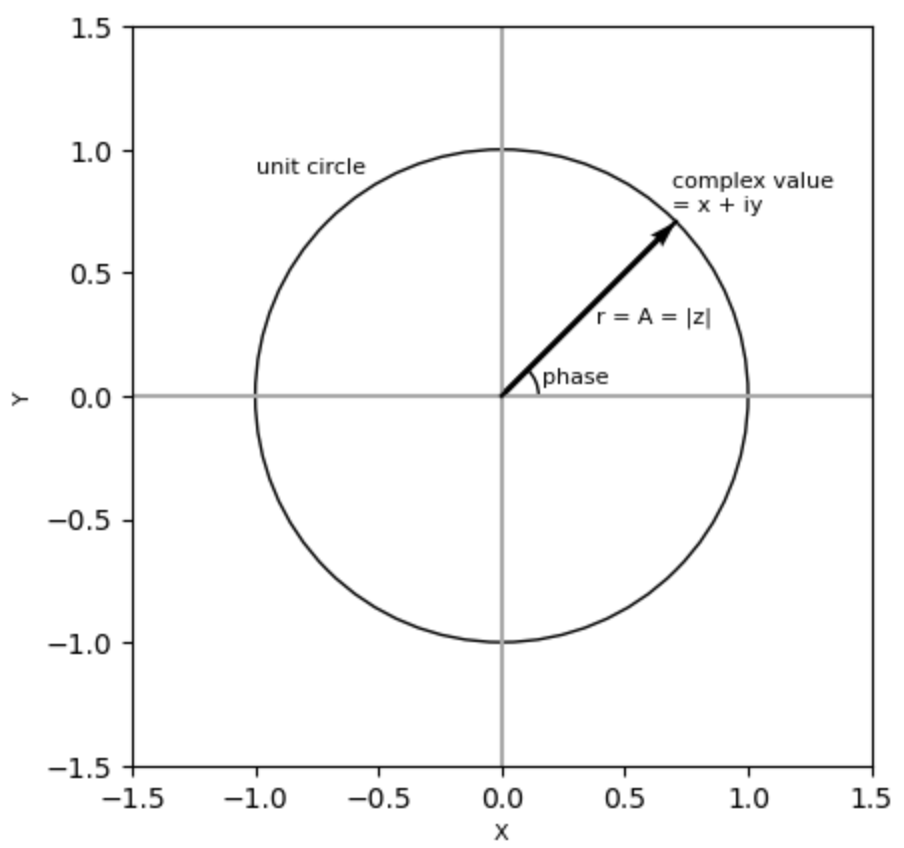
\includegraphics[width=0.5\textwidth]{figures/chapter2/complex_value.png} 
    \caption{Complex value representation.}  
    \label{fig:complex_value} 
\end{figure}

\section{Fourier transform}

A broadband signal in the time-domain has perfect temporal resolution, but does not offer any information on the different frequencies. Fourier transform moves the signal from time-domain to the frequency domain. It is defined as:

$$
F(\omega) = \int_{-\infty}^{\infty} e^{-2 \pi i \omega x} \, f(x) dx
$$

Where:

\begin{itemize}
    \item $f(x)$ is the time-domain signal, typically a function of time.
    \item $F(\omega)$ is the frequency-domain representation of the signal, where $\omega$ denotes the frequency variable. This is a complex-valued function meaning it contains both magnitude and phase information about the frequency components.
    \item $e^{-2 \pi i \omega x}$ is a complex exponential function that oscillates at frequency $\omega$. The complex form is used because it simplifies many mathematical operations.
    \item The integral $\int_{-\infty}^{\infty}$ indicates that the Fourier Transform is calculated over the entire time-domain signal.
\end{itemize}


\section{Welch's method}
Welch's method estimates the power spectral density by splitting the data into overlapping segments, calculating a modified periodogram for each segment, and then averaging the periodograms \cite{welch1967use}.

\section{Power Spectrum Density}
The PSD describes how signal power is distributed across frequencies, offering a quantitative lens into brain dynamics. Techniques like Welch's method refine PSD estimation by averaging power values across overlapping time windows, reducing noise while enhancing robustness. Wavelet-based PSD analysis extends this by accommodating the transient, non-stationary nature of neural signals. 

A key feature of neural PSDs is the \textbf{1/f scaling law}, where power diminishes with increasing frequency. This fractal characteristic underscores the hierarchical structure of brain dynamics and contextualizes prominent oscillatory peaks, such as those in the alpha and gamma bands.

\section{Wavelet Transform}
To address the stationarity challenge, wavelet transforms offer a time-frequency localization approach. The Morlet wavelet, characterized by its Gaussian envelope, provides a continuous representation of oscillatory dynamics across time and frequency. By capturing transient bursts and phase slips, wavelet analysis enhances our understanding of neural oscillatory phenomena. 

Key properties revealed through wavelet analysis include:
\begin{itemize}
\item \textbf{Amplitude}: Reflects signal strength and local synchronization levels.
\item \textbf{Phase}: Represents the oscillation's position within its cycle, critical for analyzing synchrony and cross-frequency coupling.
\end{itemize}

The Morlet wavelet with both time and frequency scaling is given by the equation:

$$
\psi(t) = A \cdot e^{-\frac{t^2}{2\sigma^2}} \cdot e^{2i \pi f_0 t} 
$$

Where:
\begin{itemize}
  \item \( \psi(t) \) is the Morlet wavelet function,
  \item \( f_0 \) is the central frequency of the wavelet (controls the frequency),
  \item \( \sigma \) is the width of the Gaussian window (controls the time localization),
  \item \( A \) is the normalization factor.
\end{itemize}



\section{Biological Realities: Bursts and Phase Slips}
Real-world oscillations deviate from idealized sine waves, manifesting as brief bursts interspersed with phase slips. These dynamic features, observable through wavelet filtering, provide insights into the brain's adaptability. For instance:
\begin{itemize}
\item \textbf{Gamma bursts} facilitate sensory processing.
\item \textbf{Alpha bursts} contribute to inhibitory control.
\end{itemize}

Wavelet analysis captures these nuances, revealing the functional significance of oscillatory bursts and their temporal stability.

\section{Practical Applications}
Combining Fourier and wavelet transforms with PSD analysis forms the cornerstone of neural signal processing. These methods are integral to studying brain dynamics via modalities like EEG and MEG, as well as intracranial techniques such as SEEG and ECoG. Practical applications include:
\begin{itemize}
\item Investigating cognitive states through alpha rhythms.
\item Linking gamma oscillations to attentional mechanisms.
\item Identifying biomarkers for neurological disorders.
\end{itemize}

\section{Conclusion}
Filtering and PSD analysis are fundamental tools for decoding the rhythmic patterns that define brain function. By dissecting oscillatory dynamics, these techniques bridge foundational neuroscience with practical applications, paving the way for innovations in understanding synchrony, connectivity, and criticality.

\vspace{10pt}           % Adds 10pt of vertical spa
\rule{\linewidth}{0.4pt} % Horizontal line
\vspace{1pt}           % Adds 10pt of vertical spa

\textbf{Questions for Review}
\begin{enumerate}
\item How does the Fourier Transform aid in isolating oscillatory components?
\item What are the advantages of wavelet analysis over traditional Fourier methods?
\item Explain the significance of the 1/f scaling law in neural PSDs.
\end{enumerate}

\textbf{Recommended Reading}
\begin{itemize}
\item Buzsáki, G. \textit{Rhythms of the Brain}. Oxford University Press, 2006.  \cite{buzsaki2006rhythms}
    \begin{itemize}
        \item Cycle 1, pages 20–45.
    \end{itemize}
\item Börgers, C., Protobook Chapter 30: Pyramidal Interneuron Network Gamma (PING). Available at: \url{https://web.njit.edu/~horacio/AdvancedCompNeuro/downloads/BorgersProtobook_Ch30_PING.pdf} \cite{borgers_ping}.
\end{itemize}
